\documentclass[9pt]{beamer}
\usepackage{graphicx}
\usepackage{enumitem}

\usetheme{metropolis}
\setbeamersize{text margin left=1.5cm, text margin right=1.5cm}
\setlist[itemize,1]{label=\small$\bullet$}
\setbeamertemplate{footline}{}
\setbeamertemplate{navigation symbols}{}

\title{CS240 Project Presentation}
\author{Mradul Sonkar (23B0980)\\ Vijaya Raghavendra (23B1042)}
\date{\today}

\begin{document}
\maketitle

\begin{frame}{Problem Statement}
    \noindent {\LARGE \textbf{Input}}\\[0.2cm]
    A time series dataset of stock market features including
    open prices, close prices, and trading volume, along with their respective
    lags.
\end{frame}

\begin{frame}{Problem Statement}
    \noindent {\LARGE \textbf{Output}}\\[0.2cm]
    A real-valued prediction representing the closing price of
    the stock in the next interval.
\end{frame}

\begin{frame}{Problem Statement}
    \noindent {\LARGE \textbf{Example}}\\[0.3cm]

    \textbf{Input:}
    \begin{table}[h!]
        \centering
        \begin{tabular}{|c|c|c|c|}
            \hline
            \textbf{Time} & \textbf{Open Price} & \textbf{Close Price} &
            \textbf{Volume}
            \\
            \hline
            $t-2$         & 101.25              & 102.10               &
            1205000                                                      \\
            $t-1$         & 102.30              & 101.80               &
            1150000                                                      \\
            $t$           & 101.90              & 102.50               &
            1234000                                                      \\
            \hline
        \end{tabular}
    \end{table}

    \textbf{Output:}\\
    \begin{center}
        Predicted Close Price at $t+1$ = \textbf{102.85}
    \end{center}

\end{frame}

\begin{frame}{Problem Statement}
    \noindent {\LARGE \textbf{Description}}\\[0.2cm]
    This project aims to build a predictive model for stock prices using
    sequential deep learning techniques. Specifically, it uses a Long
    Short-Term
    Memory (LSTM) network to capture temporal dependencies in historical price
    and
    volume data. The model is trained and evaluated using a streaming setup
    enabled
    by the \textbf{RollingRegressor} from the \textbf{deep-river} library,
    making
    it suitable for real-time or online prediction scenarios.

\end{frame}

\begin{frame}{Motivation}
    The idea for this project originated from a previously suggested stock
    market prediction task in the CS240 course, which was based on old and
    static
    historical data. The project was useful but it lacked real-time
    applicability.
    To address this gap, we aimed to develop a more relevant and practical
    system—one capable of making stock market predictions on up-to-date data in
    a
    streaming setting. This enhances both the realism and the impact of the
    problem, making it more aligned with real-world financial systems where
    timely
    decisions are crucial.
\end{frame}

\begin{frame}{Dataset}

    \noindent {\LARGE \textbf{Example}}\\[0.3cm]

    \textbf{Input:}
    \begin{table}[h!]
        \centering
        \begin{tabular}{|c|c|c|c|}
            \hline
            \textbf{Time} & \textbf{Open Price} & \textbf{Close Price} &
            \textbf{Volume}
            \\
            \hline
            $t-2$         & 101.25              & 102.10               &
            1205000                                                      \\
            $t-1$         & 102.30              & 101.80               &
            1150000                                                      \\
            $t$           & 101.90              & 102.50               &
            1234000                                                      \\
            \hline
        \end{tabular}
    \end{table}

    \textbf{Output:}\\
    \begin{center}
        Predicted Close Price at $t+1$ = \textbf{102.85}
    \end{center}
\end{frame}


\begin{frame}{Dataset}
    \noindent {\LARGE \textbf{Source}}\\[0.3cm]
    The data is collected using the \texttt{yfinance} Python API from Yahoo Finance.\\[0.15cm]
    \textbf{Citation:}
    \href{https://pypi.org/project/yfinance/}{Yahoo Finance API}

\end{frame}

\begin{frame}{Methodology}
    \noindent {\LARGE \textbf{Model Architecture}}\\[0.3cm]
    The model is a two-layer bidirectional LSTM followed by two fully connected
    layers:
    \begin{itemize}
        \item \textbf{Input:} Sequence of vectors (each with $n$ features),
              representing past timesteps
        \item \textbf{LSTM:} 2 layers, 32 hidden units per direction, dropout =
              0.2, bidirectional
        \item \textbf{Dense Layers:} A ReLU-activated hidden layer of size 32,
              followed by a final linear layer outputting a single real value
              (the predicted
              close price)
    \end{itemize}
\end{frame}

\begin{frame}{Methodology}
    \begin{figure}[htbp]
        \centering
        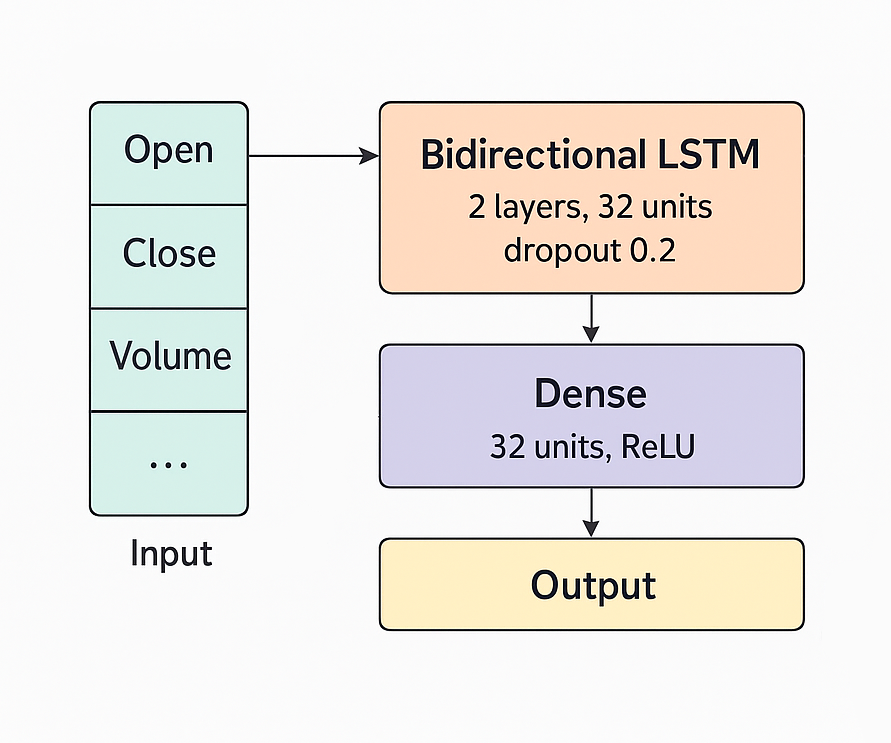
\includegraphics[width=0.8\textwidth]{model3.png}
        \caption{Model Architecture}
    \end{figure}
\end{frame}


\begin{frame}{Methodology}
    \noindent {\LARGE \textbf{Intuition}}\\[0.3cm]

    The bidirectional LSTM captures both forward and backward dependencies
    across
    the input sequence, improving pattern recognition in short-term trends. The
    dense layers enhance learning capacity and non-linearity, enabling better
    generalization over noisy stock price data.

\end{frame}

\begin{frame}{Methodology}
    \noindent {\LARGE \textbf{Implementation}}\\[0.8cm]
    \begin{description}[leftmargin=3.5cm, style=nextline]
        \item[Framework:] PyTorch
        \item[Training Strategy:] Online learning using
            \textbf{RollingRegressor}
            from \textbf{deep-river}
        \item[Loss Function:] Mean Squared Error (MSE) and Mean Absolute Error
            (MAE)
        \item[Optimizer:] Adam (learning rate = 0.001)
        \item[Features:] Lagged Open, Close, and Volume over 3 timesteps ($t$,
            $t-1$, $t-2$)
    \end{description}

\end{frame}

% \begin{frame}{Learnings}
%     \noindent {\LARGE \textbf{Technical Learnings}}\\[0.3cm]
%         Through this project, we gained in-depth experience with time series forecasting, particularly using LSTM (Long Short-Term Memory) networks. We learned how to preprocess financial data, integrate multiple features such as open, close, and volume prices, and handle issues related to missing data and noise. We also learnt using libraries like \textbf{PyTorch} for implementing neural networks and \textbf{deep_rive} rolling regressors for real-time prediction.
% \end{frame}

\begin{frame}{Learnings}
    \noindent {\LARGE \textbf{Technical Learnings}}\\[0.3cm]
    Through this project, we gained in-depth experience with time series forecasting, particularly using LSTM (Long Short-Term Memory) networks. We learned how to preprocess financial data, integrate multiple features such as open, close, and volume prices, and handle issues related to missing data and noise. We also learnt using libraries like \textbf{PyTorch} for implementing neural networks and \textbf{deep-river} rolling regressors for real-time prediction.
\end{frame}

\begin{frame}{Learnings}
    \noindent {\LARGE \textbf{Problem-Solving}}\\[0.3cm]
    We learned how to approach real-world problems where data is dynamic, unstructured, and noisy. Addressing issues like overfitting, underfitting, and hyperparameter tuning taught us the importance of balancing model complexity with performance. Experimenting with different architectures (e.g., bidirectional LSTMs) enhanced my problem-solving skills in a dynamic and unpredictable environment like the stock market.
\end{frame}

\begin{frame}{Learnings}
    \noindent {\LARGE \textbf{Experimentation}}\\[0.3cm]
    The project involved continuous experimentation with model parameters, training strategies, and input features to improve prediction accuracy. I learned the importance of tracking results, analyzing errors, and refining hypotheses to iterate toward the best solution. This experimental mindset is essential for refining machine learning models and optimizing them for deployment.
\end{frame}

\begin{frame}[c]
    \centering
    {\Huge \textbf{Thank You!}}\\[1cm]
\end{frame}


\end{document}